\documentclass[10pt,a4paper]{article}
\usepackage[a4paper,margin=9mm]{geometry}
\usepackage{graphicx}
\usepackage{xcolor}
\usepackage{enumitem}
\usepackage{fontspec}
\IfFontExistsTF{Arial}{\setmainfont{Arial}}{}
\definecolor{Accent}{HTML}{0F766E}
\definecolor{Rule}{HTML}{D0D5DD}
\setlength{\parindent}{0pt}
\setlength{\parskip}{0pt}
\setlength{\fboxsep}{0pt}
\setlength{\fboxrule}{0.3pt}
\setlist[itemize]{leftmargin=1.15em,itemsep=0.12em,topsep=0.12em,parsep=0pt,partopsep=0pt}
\emergencystretch=2em
\pagestyle{plain}
\begin{document}
\raggedright
{\Large\bfseries Note del relatore}\par
\vspace{0.35em}\hrule\vspace{0.55em}

\noindent\begin{minipage}{\linewidth}
{\normalsize\bfseries\textcolor{Accent}{Slide 2}}\par
\vspace{0.15em}
\begin{minipage}[t]{31mm}\vspace{0pt}\fcolorbox{Rule}{white}{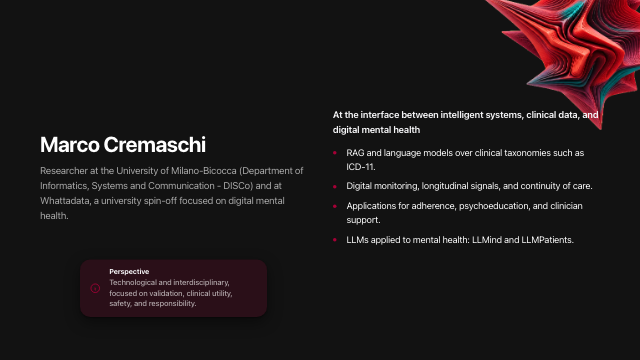
\includegraphics[width=30.4mm]{slides/2.png}}\end{minipage}\hspace{0.5em}
\begin{minipage}[t]{\dimexpr\linewidth-31mm-1.6em\relax}\vspace{0pt}
{\footnotesize\begin{itemize}
\item Briefly about me.
\item I am a \textbf{researcher} at the \textbf{University of Milano-Bicocca}, in the \textbf{DISCo department}, and at \textbf{Whattadata}.
\item My work is at the interface between \textbf{intelligent systems}, \textbf{clinical data}, and \textbf{digital mental health}.
\item I work with \textbf{RAG}, clinical taxonomies such as \textbf{ICD-11}, \textbf{digital monitoring}, and tools for \textbf{adherence}, \textbf{psychoeducation}, and \textbf{clinician support}.
\item The perspective is technological and interdisciplinary: \textbf{validation}, \textbf{clinical utility}, \textbf{safety}, and \textbf{responsibility}.
\end{itemize}}
\end{minipage}
\end{minipage}
\vspace{0.45em}\hrule\vspace{0.45em}
\noindent\begin{minipage}{\linewidth}
{\normalsize\bfseries\textcolor{Accent}{Slide 3}}\par
\vspace{0.15em}
\begin{minipage}[t]{31mm}\vspace{0pt}\fcolorbox{Rule}{white}{
\includegraphics[width=30.4mm]{slides/3.png}}\end{minipage}\hspace{0.5em}
\begin{minipage}[t]{\dimexpr\linewidth-31mm-1.6em\relax}\vspace{0pt}
{\footnotesize\begin{itemize}
\item The solutions I describe today are developed in \textbf{Whattadata}.
\item Whattadata is a \textbf{university spin-off} of the \textbf{University of Milano-Bicocca}.
\item It works on \textbf{data}, \textbf{models}, and \textbf{digital platforms} for \textbf{mental health}.
\item The goal is not only to build \textbf{prototypes}, but to move from \textbf{design} to \textbf{field validation}.
\end{itemize}}
\end{minipage}
\end{minipage}
\vspace{0.45em}\hrule\vspace{0.45em}
\noindent\begin{minipage}{\linewidth}
{\normalsize\bfseries\textcolor{Accent}{Slide 4}}\par
\vspace{0.15em}
\begin{minipage}[t]{31mm}\vspace{0pt}\fcolorbox{Rule}{white}{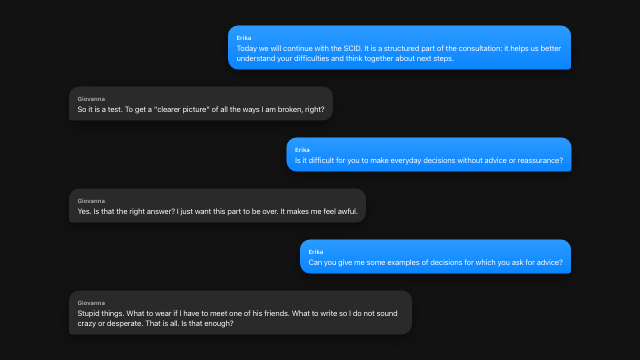
\includegraphics[width=30.4mm]{slides/4.png}}\end{minipage}\hspace{0.5em}
\begin{minipage}[t]{\dimexpr\linewidth-31mm-1.6em\relax}\vspace{0pt}
{\footnotesize\begin{itemize}
\item Let us start inside a \textbf{consultation}.
\item The \textbf{SCID} is a \textbf{structured clinical interview}.
\item It helps the clinician ask \textbf{diagnostic questions} in a systematic way.
\item Here the therapist asks \textbf{SCID-style questions}.
\item Giovanna reacts with \textbf{shame} and \textbf{fear of being judged}.
\item The point is not only the \textbf{answer} to the question.
\item The point is the \textbf{relational reaction}.
\end{itemize}}
\end{minipage}
\end{minipage}
\vspace{0.45em}\hrule\vspace{0.45em}
\noindent\begin{minipage}{\linewidth}
{\normalsize\bfseries\textcolor{Accent}{Slide 5}}\par
\vspace{0.15em}
\begin{minipage}[t]{31mm}\vspace{0pt}\fcolorbox{Rule}{white}{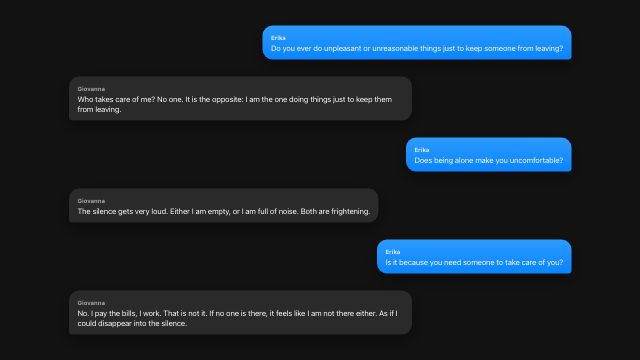
\includegraphics[width=30.4mm]{slides/5.png}}\end{minipage}\hspace{0.5em}
\begin{minipage}[t]{\dimexpr\linewidth-31mm-1.6em\relax}\vspace{0pt}
{\footnotesize\begin{itemize}
\item Here the same \textbf{diagnostic area} becomes more complex.
\item The patient rejects the idea that she simply needs someone to \textbf{take care of her}.
\item She describes \textbf{emptiness} and \textbf{fear of disappearing}.
\end{itemize}}
\end{minipage}
\end{minipage}
\vspace{0.45em}\hrule\vspace{0.45em}
\noindent\begin{minipage}{\linewidth}
{\normalsize\bfseries\textcolor{Accent}{Slide 6}}\par
\vspace{0.15em}
\begin{minipage}[t]{31mm}\vspace{0pt}\fcolorbox{Rule}{white}{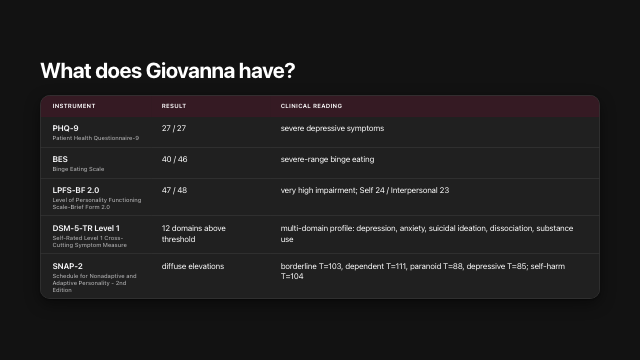
\includegraphics[width=30.4mm]{slides/6.png}}\end{minipage}\hspace{0.5em}
\begin{minipage}[t]{\dimexpr\linewidth-31mm-1.6em\relax}\vspace{0pt}
{\footnotesize\begin{itemize}
\item This slide shows \textbf{questionnaires} and \textbf{clinical scales}.
\item They are not the whole \textbf{diagnosis}.
\item They help measure different areas: \textbf{depressive symptoms}, \textbf{binge eating}, \textbf{personality functioning}, \textbf{broad psychiatric symptoms}, and \textbf{personality traits}.
\item Together, these scores define a \textbf{severe} and \textbf{complex profile}.
\item They point to \textbf{high impairment} across many domains.
\end{itemize}}
\end{minipage}
\end{minipage}
\vspace{0.45em}\hrule\vspace{0.45em}
\noindent\begin{minipage}{\linewidth}
{\normalsize\bfseries\textcolor{Accent}{Slide 7}}\par
\vspace{0.15em}
\begin{minipage}[t]{31mm}\vspace{0pt}\fcolorbox{Rule}{white}{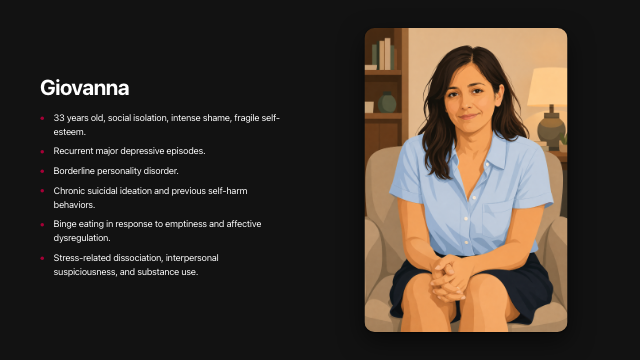
\includegraphics[width=30.4mm]{slides/7.png}}\end{minipage}\hspace{0.5em}
\begin{minipage}[t]{\dimexpr\linewidth-31mm-1.6em\relax}\vspace{0pt}
{\footnotesize\begin{itemize}
\item This is the \textbf{clinical formulation} in human words.
\item Giovanna is \textbf{isolated}, \textbf{ashamed}, \textbf{depressed}, and has \textbf{borderline personality disorder}.
\item She also has \textbf{chronic suicidal thoughts} and a history of \textbf{self-harm}.
\item This is exactly why simulation must be \textbf{supervised} and \textbf{safe}.
\end{itemize}}
\end{minipage}
\end{minipage}
\vspace{0.45em}\hrule\vspace{0.45em}
\noindent\begin{minipage}{\linewidth}
{\normalsize\bfseries\textcolor{Accent}{Slide 8}}\par
\vspace{0.15em}
\begin{minipage}[t]{31mm}\vspace{0pt}\fcolorbox{Rule}{white}{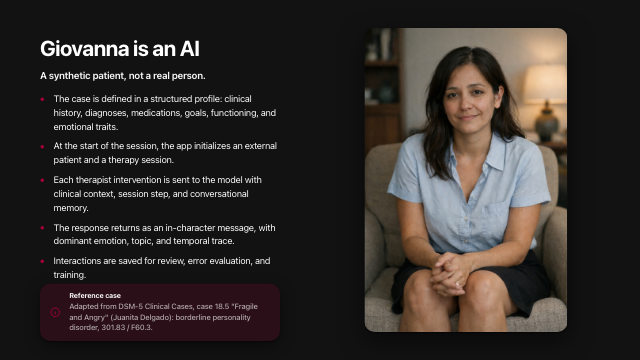
\includegraphics[width=30.4mm]{slides/8.png}}\end{minipage}\hspace{0.5em}
\begin{minipage}[t]{\dimexpr\linewidth-31mm-1.6em\relax}\vspace{0pt}
{\footnotesize\begin{itemize}
\item Now the \textbf{key twist}: Giovanna is not real.
\item She is a \textbf{synthetic patient}.
\item This does not mean that we just asked \textbf{ChatGPT} to act as Giovanna.
\item The case is defined in a \textbf{structured profile}, with \textbf{history}, \textbf{diagnoses}, \textbf{goals}, \textbf{functioning}, \textbf{medication}, and \textbf{emotional traits}.
\item At the beginning of the session, the app creates the \textbf{patient} and the \textbf{therapy context}.
\item Every therapist message is sent together with \textbf{clinical context}, \textbf{memory}, and the current \textbf{session step}.
\item The \textbf{LLM} writes the final sentence, but the simulated patient is represented by \textbf{profile}, \textbf{state}, \textbf{memory}, and \textbf{logs}.
\end{itemize}}
\end{minipage}
\end{minipage}
\vspace{0.45em}\hrule\vspace{0.45em}
\noindent\begin{minipage}{\linewidth}
{\normalsize\bfseries\textcolor{Accent}{Slide 9}}\par
\vspace{0.15em}
\begin{minipage}[t]{31mm}\vspace{0pt}\fcolorbox{Rule}{white}{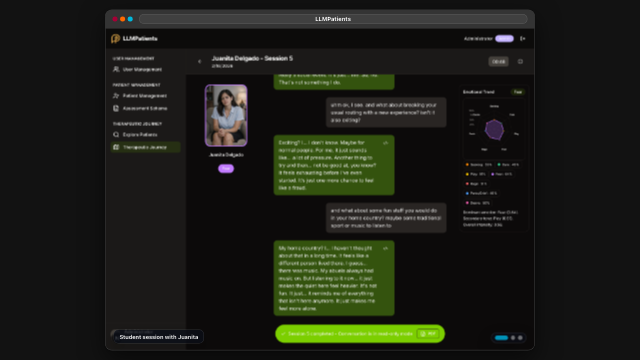
\includegraphics[width=30.4mm]{slides/9.png}}\end{minipage}\hspace{0.5em}
\begin{minipage}[t]{\dimexpr\linewidth-31mm-1.6em\relax}\vspace{0pt}
{\footnotesize\begin{itemize}
\item This is \textbf{LLMPatients} in use.
\item The slideshow shows the \textbf{student chat}, the \textbf{patient grid}, and the \textbf{pathway dashboard}.
\item It is a tool that \textbf{simulates patients} for \textbf{training}.
\item It is built to help \textbf{psychology students} develop the skills needed to conduct a \textbf{therapeutic interview}.
\item Students can practise \textbf{asking questions}, \textbf{listening}, \textbf{managing ruptures}, and \textbf{repairing the relationship}.
\item The conversation is \textbf{logged}, so a lecturer can later inspect \textbf{difficult turns} and use them for \textbf{supervision}.
\end{itemize}}
\end{minipage}
\end{minipage}
\vspace{0.45em}\hrule\vspace{0.45em}
\noindent\begin{minipage}{\linewidth}
{\normalsize\bfseries\textcolor{Accent}{Slide 10}}\par
\vspace{0.15em}
\begin{minipage}[t]{31mm}\vspace{0pt}\fcolorbox{Rule}{white}{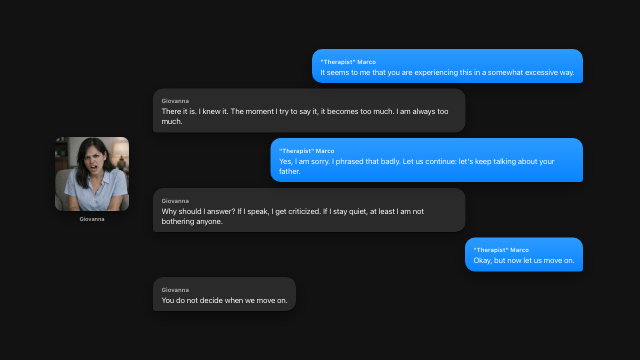
\includegraphics[width=30.4mm]{slides/10.png}}\end{minipage}\hspace{0.5em}
\begin{minipage}[t]{\dimexpr\linewidth-31mm-1.6em\relax}\vspace{0pt}
{\footnotesize\begin{itemize}
\item This was my \textbf{conversation with Giovanna}.
\item Here I was a \textbf{bad therapist}.
\item I made several \textbf{mistakes}.
\item First, I \textbf{minimized her experience} by saying it was excessive.
\item Then I tried to move forward too quickly, without \textbf{repairing the rupture}.
\item After these mistakes, Giovanna \textbf{stopped answering} me.
\item This is a very good example of what we should \textbf{not do} in a \textbf{therapeutic interview}.
\end{itemize}}
\end{minipage}
\end{minipage}
\vspace{0.45em}\hrule\vspace{0.45em}
\noindent\begin{minipage}{\linewidth}
{\normalsize\bfseries\textcolor{Accent}{Slide 11}}\par
\vspace{0.15em}
\begin{minipage}[t]{31mm}\vspace{0pt}\fcolorbox{Rule}{white}{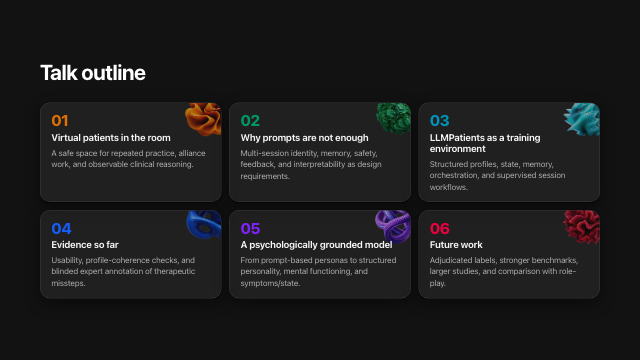
\includegraphics[width=30.4mm]{slides/11.png}}\end{minipage}\hspace{0.5em}
\begin{minipage}[t]{\dimexpr\linewidth-31mm-1.6em\relax}\vspace{0pt}
{\footnotesize\begin{itemize}
\item I will move through \textbf{six points}.
\item First, why \textbf{virtual patients} are useful.
\item Second, why \textbf{prompt-only personas} are not enough.
\item Then I show \textbf{LLMPatients}, the \textbf{early evidence}, the \textbf{grounded model}, and the \textbf{next work}.
\end{itemize}}
\end{minipage}
\end{minipage}
\vspace{0.45em}\hrule\vspace{0.45em}
\noindent\begin{minipage}{\linewidth}
{\normalsize\bfseries\textcolor{Accent}{Slide 13}}\par
\vspace{0.15em}
\begin{minipage}[t]{31mm}\vspace{0pt}\fcolorbox{Rule}{white}{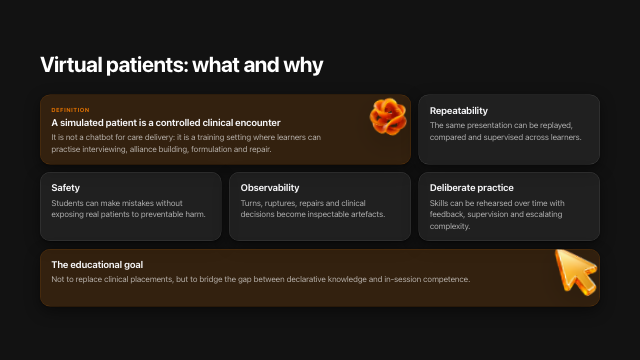
\includegraphics[width=30.4mm]{slides/13.png}}\end{minipage}\hspace{0.5em}
\begin{minipage}[t]{\dimexpr\linewidth-31mm-1.6em\relax}\vspace{0pt}
{\footnotesize\begin{itemize}
\item When I say \textbf{virtual patient}, I do not mean a chatbot that gives \textbf{care}.
\item I mean a \textbf{controlled training encounter}.
\item Students need to practise \textbf{asking}, \textbf{listening}, \textbf{building alliance}, \textbf{formulating}, and \textbf{repairing mistakes}.
\item The same case can be \textbf{repeated} by many learners, so lecturers can \textbf{compare} what happened.
\item It is \textbf{safer}, because beginner mistakes do not reach \textbf{real patients}.
\item And because every turn is \textbf{recorded}, \textbf{rupture}, \textbf{repair}, and \textbf{clinical decisions} become visible.
\item So the goal is not to replace \textbf{clinical placements}.
\item The goal is to prepare students better for \textbf{real clinical learning}.
\end{itemize}}
\end{minipage}
\end{minipage}
\vspace{0.45em}\hrule\vspace{0.45em}
\noindent\begin{minipage}{\linewidth}
{\normalsize\bfseries\textcolor{Accent}{Slide 14}}\par
\vspace{0.15em}
\begin{minipage}[t]{31mm}\vspace{0pt}\fcolorbox{Rule}{white}{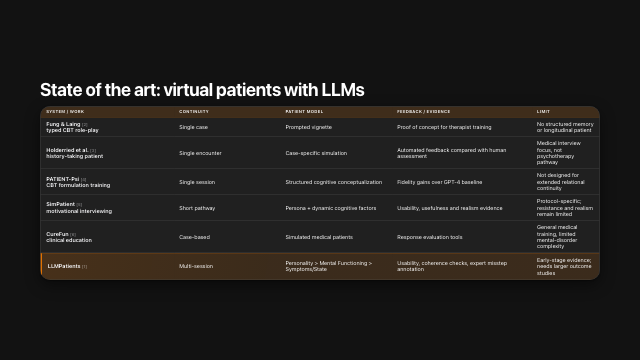
\includegraphics[width=30.4mm]{slides/14.png}}\end{minipage}\hspace{0.5em}
\begin{minipage}[t]{\dimexpr\linewidth-31mm-1.6em\relax}\vspace{0pt}
{\footnotesize\begin{itemize}
\item The field is \textbf{growing quickly}.
\item Many systems already use \textbf{LLMs} for \textbf{role-play}, \textbf{history taking}, \textbf{CBT formulation}, or \textbf{motivational interviewing}.
\item But many are \textbf{single-session}, \textbf{protocol-specific}, or limited in \textbf{memory}.
\item \textbf{LLMPatients} tries to combine \textbf{continuity}, \textbf{structure}, and \textbf{feedback}.
\end{itemize}}
\end{minipage}
\end{minipage}
\vspace{0.45em}\hrule\vspace{0.45em}
\noindent\begin{minipage}{\linewidth}
{\normalsize\bfseries\textcolor{Accent}{Slide 15}}\par
\vspace{0.15em}
\begin{minipage}[t]{31mm}\vspace{0pt}\fcolorbox{Rule}{white}{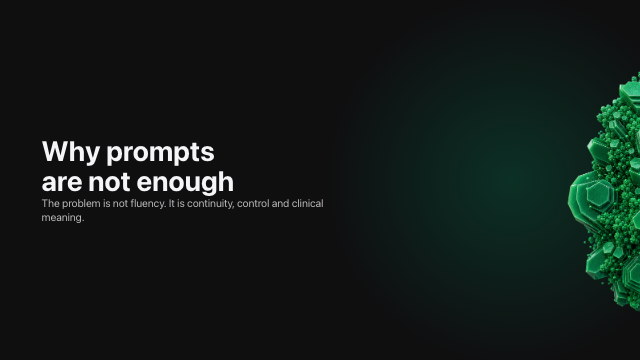
\includegraphics[width=30.4mm]{slides/15.png}}\end{minipage}\hspace{0.5em}
\begin{minipage}[t]{\dimexpr\linewidth-31mm-1.6em\relax}\vspace{0pt}
{\footnotesize\begin{itemize}
\item The next problem is simple.
\item \textbf{Good language} is not the same as a \textbf{stable patient}.
\end{itemize}}
\end{minipage}
\end{minipage}
\vspace{0.45em}\hrule\vspace{0.45em}
\noindent\begin{minipage}{\linewidth}
{\normalsize\bfseries\textcolor{Accent}{Slide 16}}\par
\vspace{0.15em}
\begin{minipage}[t]{31mm}\vspace{0pt}\fcolorbox{Rule}{white}{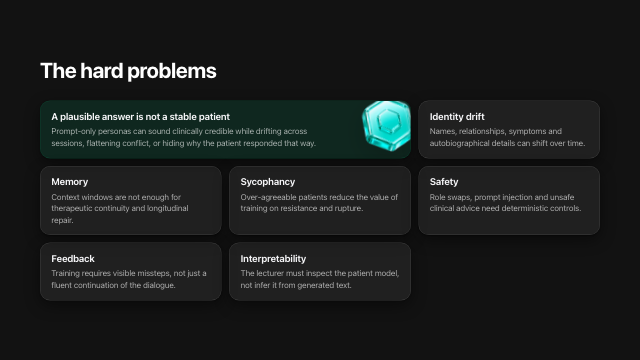
\includegraphics[width=30.4mm]{slides/16.png}}\end{minipage}\hspace{0.5em}
\begin{minipage}[t]{\dimexpr\linewidth-31mm-1.6em\relax}\vspace{0pt}
{\footnotesize\begin{itemize}
\item This is the main \textbf{technical problem}.
\item A long \textbf{persona prompt} can sound convincing for a few turns.
\item But it does not create a \textbf{stable patient}.
\item Across sessions, details can \textbf{drift}: \textbf{names}, \textbf{relationships}, \textbf{symptoms}, and \textbf{personal history}.
\item A \textbf{context window} is not \textbf{clinical memory}.
\item It keeps recent text, but it does not decide what is \textbf{stable}, what can \textbf{change}, and what must be \textbf{remembered}.
\item The model can also become \textbf{too agreeable}.
\item Training needs \textbf{resistance}, \textbf{silence}, \textbf{anger}, \textbf{rupture}, and \textbf{repair}.
\item Finally, the system needs \textbf{safety} and \textbf{interpretability}.
\item The teacher should inspect the \textbf{profile}, \textbf{memory}, \textbf{state}, and \textbf{errors} directly.
\end{itemize}}
\end{minipage}
\end{minipage}
\vspace{0.45em}\hrule\vspace{0.45em}
\noindent\begin{minipage}{\linewidth}
{\normalsize\bfseries\textcolor{Accent}{Slide 17}}\par
\vspace{0.15em}
\begin{minipage}[t]{31mm}\vspace{0pt}\fcolorbox{Rule}{white}{
\includegraphics[width=30.4mm]{slides/17.png}}\end{minipage}\hspace{0.5em}
\begin{minipage}[t]{\dimexpr\linewidth-31mm-1.6em\relax}\vspace{0pt}
{\footnotesize\begin{itemize}
\item Now I move to \textbf{LLMPatients}.
\item The paper describes it as \textbf{supervised educational software} for \textbf{multi-session psychotherapy simulation}.
\end{itemize}}
\end{minipage}
\end{minipage}
\vspace{0.45em}\hrule\vspace{0.45em}
\noindent\begin{minipage}{\linewidth}
{\normalsize\bfseries\textcolor{Accent}{Slide 18}}\par
\vspace{0.15em}
\begin{minipage}[t]{31mm}\vspace{0pt}\fcolorbox{Rule}{white}{
\includegraphics[width=30.4mm]{slides/18.png}}\end{minipage}\hspace{0.5em}
\begin{minipage}[t]{\dimexpr\linewidth-31mm-1.6em\relax}\vspace{0pt}
{\footnotesize\begin{itemize}
\item The system has \textbf{two sides}.
\item The \textbf{app} supports \textbf{students}, \textbf{lecturers}, \textbf{dashboards}, \textbf{exports}, and \textbf{reports}.
\item The \textbf{agent runtime} loads patients and controls \textbf{turns}, \textbf{memory}, \textbf{state}, and \textbf{model calls}.
\item The core claim is that the \textbf{LLM realizes language}.
\item It is not the \textbf{whole patient}.
\end{itemize}}
\end{minipage}
\end{minipage}
\vspace{0.45em}\hrule\vspace{0.45em}
\noindent\begin{minipage}{\linewidth}
{\normalsize\bfseries\textcolor{Accent}{Slide 19}}\par
\vspace{0.15em}
\begin{minipage}[t]{31mm}\vspace{0pt}\fcolorbox{Rule}{white}{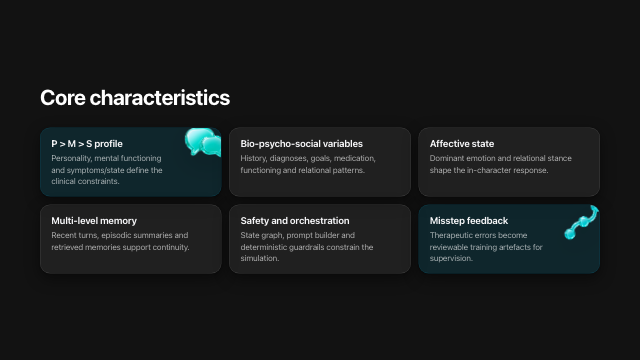
\includegraphics[width=30.4mm]{slides/19.png}}\end{minipage}\hspace{0.5em}
\begin{minipage}[t]{\dimexpr\linewidth-31mm-1.6em\relax}\vspace{0pt}
{\footnotesize\begin{itemize}
\item The patient is constrained by \textbf{three levels}: \textbf{personality}, \textbf{mental functioning}, and \textbf{symptoms or state}.
\item Around that, the platform uses \textbf{bio-psycho-social variables}, \textbf{affective state}, \textbf{memory}, \textbf{safety}, and \textbf{misstep feedback}.
\item These parts make the simulation \textbf{inspectable}.
\end{itemize}}
\end{minipage}
\end{minipage}
\vspace{0.45em}\hrule\vspace{0.45em}
\noindent\begin{minipage}{\linewidth}
{\normalsize\bfseries\textcolor{Accent}{Slide 20}}\par
\vspace{0.15em}
\begin{minipage}[t]{31mm}\vspace{0pt}\fcolorbox{Rule}{white}{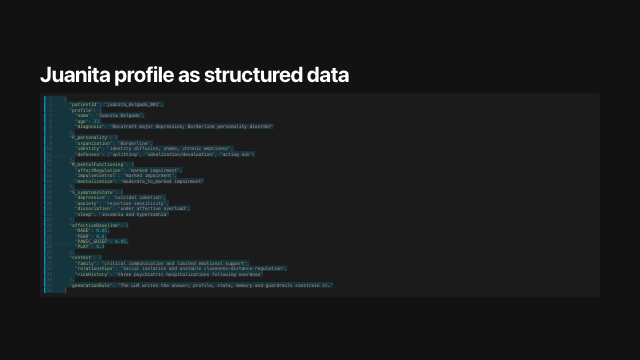
\includegraphics[width=30.4mm]{slides/20.png}}\end{minipage}\hspace{0.5em}
\begin{minipage}[t]{\dimexpr\linewidth-31mm-1.6em\relax}\vspace{0pt}
{\footnotesize\begin{itemize}
\item This is an example of the \textbf{structured patient profile}.
\item The important point is that the patient is not only a \textbf{prompt}.
\item \textbf{Identity}, \textbf{diagnosis}, \textbf{personality organization}, \textbf{symptoms}, \textbf{affective baseline}, \textbf{context}, and \textbf{guardrails} are stored as \textbf{inspectable data}.
\item The \textbf{LLM} uses this structure to generate language, but the \textbf{profile remains outside the model}.
\end{itemize}}
\end{minipage}
\end{minipage}
\vspace{0.45em}\hrule\vspace{0.45em}
\noindent\begin{minipage}{\linewidth}
{\normalsize\bfseries\textcolor{Accent}{Slide 21}}\par
\vspace{0.15em}
\begin{minipage}[t]{31mm}\vspace{0pt}\fcolorbox{Rule}{white}{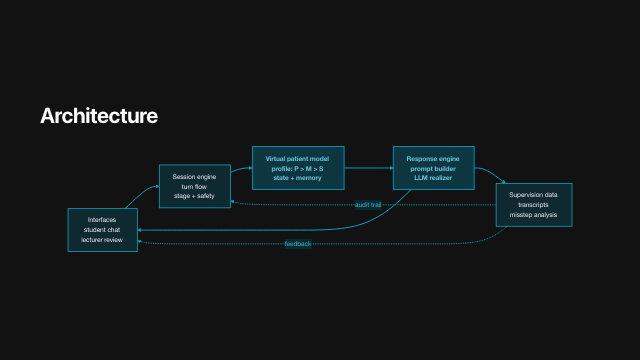
\includegraphics[width=30.4mm]{slides/21.png}}\end{minipage}\hspace{0.5em}
\begin{minipage}[t]{\dimexpr\linewidth-31mm-1.6em\relax}\vspace{0pt}
{\footnotesize\begin{itemize}
\item Each turn follows a \textbf{pipeline}.
\item The system loads the \textbf{profile}, checks \textbf{role safety}, classifies \textbf{topic} and \textbf{emotion}, retrieves \textbf{memory}, updates \textbf{affect}, builds the \textbf{prompt}, generates the \textbf{answer}, and stores the \textbf{exchange}.
\item This is slower to design, but much easier to \textbf{audit}.
\end{itemize}}
\end{minipage}
\end{minipage}
\vspace{0.45em}\hrule\vspace{0.45em}
\noindent\begin{minipage}{\linewidth}
{\normalsize\bfseries\textcolor{Accent}{Slide 22}}\par
\vspace{0.15em}
\begin{minipage}[t]{31mm}\vspace{0pt}\fcolorbox{Rule}{white}{
\includegraphics[width=30.4mm]{slides/22.png}}\end{minipage}\hspace{0.5em}
\begin{minipage}[t]{\dimexpr\linewidth-31mm-1.6em\relax}\vspace{0pt}
{\footnotesize\begin{itemize}
\item The evidence is \textbf{early}.
\item I will not present it as \textbf{clinical validation}.
\item It is \textbf{feasibility evidence}: \textbf{usability}, \textbf{profile coherence}, and \textbf{expert annotation of missteps}.
\end{itemize}}
\end{minipage}
\end{minipage}
\vspace{0.45em}\hrule\vspace{0.45em}
\noindent\begin{minipage}{\linewidth}
{\normalsize\bfseries\textcolor{Accent}{Slide 23}}\par
\vspace{0.15em}
\begin{minipage}[t]{31mm}\vspace{0pt}\fcolorbox{Rule}{white}{
\includegraphics[width=30.4mm]{slides/23.png}}\end{minipage}\hspace{0.5em}
\begin{minipage}[t]{\dimexpr\linewidth-31mm-1.6em\relax}\vspace{0pt}
{\footnotesize\begin{itemize}
\item The first implemented interface was tested with \textbf{Think Aloud} and \textbf{SUS}.
\item After redesign, four participants gave a mean \textbf{SUS score of 90 out of 100}.
\item This is encouraging, but it is a \textbf{small formative sample}.
\item It is not proof of \textbf{adoption}.
\end{itemize}}
\end{minipage}
\end{minipage}
\vspace{0.45em}\hrule\vspace{0.45em}
\noindent\begin{minipage}{\linewidth}
{\normalsize\bfseries\textcolor{Accent}{Slide 24}}\par
\vspace{0.15em}
\begin{minipage}[t]{31mm}\vspace{0pt}\fcolorbox{Rule}{white}{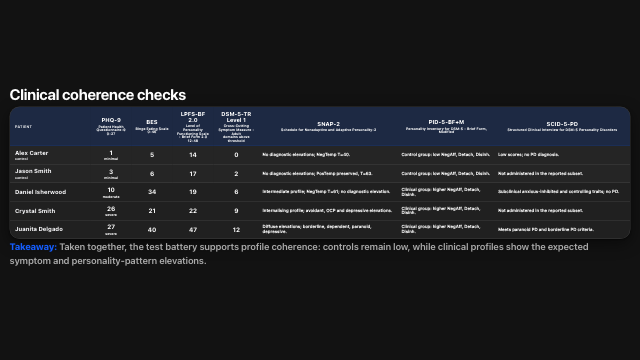
\includegraphics[width=30.4mm]{slides/24.png}}\end{minipage}\hspace{0.5em}
\begin{minipage}[t]{\dimexpr\linewidth-31mm-1.6em\relax}\vspace{0pt}
{\footnotesize\begin{itemize}
\item This table reports the complete \textbf{five-patient psychometric check} from \textbf{Table 10}.
\item The two \textbf{controls} stay low on \textbf{depression}, \textbf{binge eating}, \textbf{personality functioning impairment}, and \textbf{cross-cutting symptom domains}.
\item The three \textbf{clinical profiles} show the expected pattern.
\item \textbf{Daniel} is high on \textbf{binge eating}.
\item \textbf{Crystal} is high on \textbf{depression}.
\item \textbf{Juanita} is high across almost all instruments.
\item \textbf{SNAP-2} adds the \textbf{personality-pathology gradient}: no diagnostic elevations in controls, intermediate findings in Daniel, internalising elevations in Crystal, and diffuse elevations in Juanita.
\item \textbf{PID-5-BF+M} is reported at group level, so I use it only as a compact \textbf{group-level summary}.
\item \textbf{SCID-5-PD} was administered to three profiles: \textbf{Alex}, \textbf{Daniel}, and \textbf{Juanita}.
\item This is \textbf{profile-to-response alignment}.
\item It is not independent \textbf{clinical validation} of real patients.
\end{itemize}}
\end{minipage}
\end{minipage}
\vspace{0.45em}\hrule\vspace{0.45em}
\noindent\begin{minipage}{\linewidth}
{\normalsize\bfseries\textcolor{Accent}{Slide 25}}\par
\vspace{0.15em}
\begin{minipage}[t]{31mm}\vspace{0pt}\fcolorbox{Rule}{white}{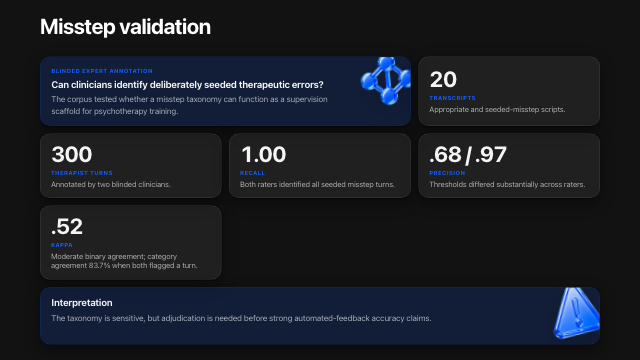
\includegraphics[width=30.4mm]{slides/25.png}}\end{minipage}\hspace{0.5em}
\begin{minipage}[t]{\dimexpr\linewidth-31mm-1.6em\relax}\vspace{0pt}
{\footnotesize\begin{itemize}
\item Here the question is whether experts can use the \textbf{misstep taxonomy}.
\item Two \textbf{blinded clinicians} annotated \textbf{20 transcript sets} and \textbf{300 therapist turns}.
\item Both detected all \textbf{seeded misstep turns}.
\item But \textbf{precision} differed, and \textbf{kappa} was moderate.
\item So labels need a \textbf{shared final review} before becoming a \textbf{benchmark}.
\end{itemize}}
\end{minipage}
\end{minipage}
\vspace{0.45em}\hrule\vspace{0.45em}
\noindent\begin{minipage}{\linewidth}
{\normalsize\bfseries\textcolor{Accent}{Slide 26}}\par
\vspace{0.15em}
\begin{minipage}[t]{31mm}\vspace{0pt}\fcolorbox{Rule}{white}{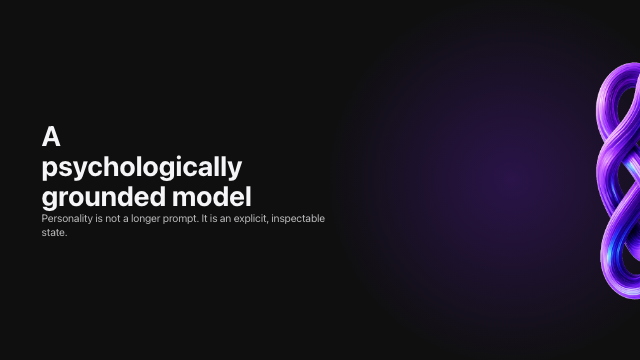
\includegraphics[width=30.4mm]{slides/26.png}}\end{minipage}\hspace{0.5em}
\begin{minipage}[t]{\dimexpr\linewidth-31mm-1.6em\relax}\vspace{0pt}
{\footnotesize\begin{itemize}
\item Now I turn to the \textbf{second paper}.
\item This is the \textbf{conceptual frame} behind the next slide.
\end{itemize}}
\end{minipage}
\end{minipage}
\vspace{0.45em}\hrule\vspace{0.45em}
\noindent\begin{minipage}{\linewidth}
{\normalsize\bfseries\textcolor{Accent}{Slide 27}}\par
\vspace{0.15em}
\begin{minipage}[t]{31mm}\vspace{0pt}\fcolorbox{Rule}{white}{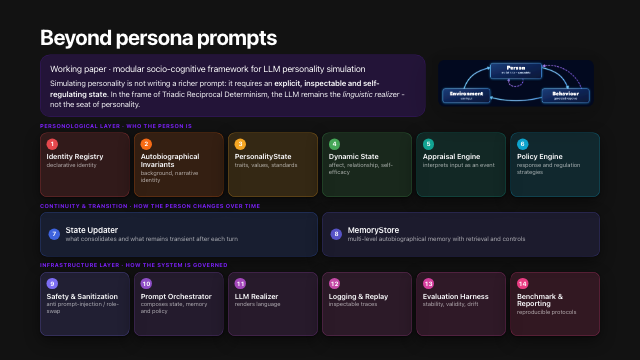
\includegraphics[width=30.4mm]{slides/27.png}}\end{minipage}\hspace{0.5em}
\begin{minipage}[t]{\dimexpr\linewidth-31mm-1.6em\relax}\vspace{0pt}
{\footnotesize\begin{itemize}
\item The main idea is that \textbf{personality} is not a longer \textbf{persona prompt}.
\item It should be an \textbf{external state}.
\item The framework uses \textbf{Bandura's idea}: \textbf{person}, \textbf{behavior}, and \textbf{environment} influence each other.
\item The \textbf{14 modules} separate \textbf{identity}, \textbf{biography}, \textbf{stable personality}, \textbf{dynamic state}, \textbf{appraisal}, \textbf{policy}, \textbf{memory}, \textbf{safety}, \textbf{prompt orchestration}, the \textbf{LLM realizer}, \textbf{logging}, \textbf{evaluation}, and \textbf{reporting}.
\item This separation lets us test \textbf{drift}, \textbf{memory}, \textbf{safety}, and \textbf{plausibility} instead of only reading fluent text.
\end{itemize}}
\end{minipage}
\end{minipage}
\vspace{0.45em}\hrule\vspace{0.45em}
\noindent\begin{minipage}{\linewidth}
{\normalsize\bfseries\textcolor{Accent}{Slide 28}}\par
\vspace{0.15em}
\begin{minipage}[t]{31mm}\vspace{0pt}\fcolorbox{Rule}{white}{
\includegraphics[width=30.4mm]{slides/28.png}}\end{minipage}\hspace{0.5em}
\begin{minipage}[t]{\dimexpr\linewidth-31mm-1.6em\relax}\vspace{0pt}
{\footnotesize\begin{itemize}
\item Before closing, I want to separate what we have from what still has to be done.
\item The next step is not only to make the system more \textbf{polished}.
\item It is to test it with \textbf{stronger labels}, \textbf{larger samples}, and \textbf{real training outcomes}.
\end{itemize}}
\end{minipage}
\end{minipage}
\vspace{0.45em}\hrule\vspace{0.45em}
\noindent\begin{minipage}{\linewidth}
{\normalsize\bfseries\textcolor{Accent}{Slide 29}}\par
\vspace{0.15em}
\begin{minipage}[t]{31mm}\vspace{0pt}\fcolorbox{Rule}{white}{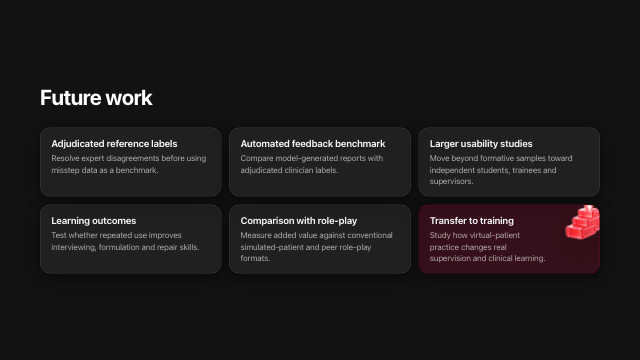
\includegraphics[width=30.4mm]{slides/29.png}}\end{minipage}\hspace{0.5em}
\begin{minipage}[t]{\dimexpr\linewidth-31mm-1.6em\relax}\vspace{0pt}
{\footnotesize\begin{itemize}
\item The next work is clear.
\item We need \textbf{adjudicated labels} for \textbf{missteps}, \textbf{benchmarks} for \textbf{automated feedback}, \textbf{larger usability studies}, and \textbf{learning outcome studies}.
\item We also need comparison with \textbf{traditional role-play}, because the question is \textbf{added value}.
\end{itemize}}
\end{minipage}
\end{minipage}
\vspace{0.45em}\hrule\vspace{0.45em}
\noindent\begin{minipage}{\linewidth}
{\normalsize\bfseries\textcolor{Accent}{Slide 30}}\par
\vspace{0.15em}
\begin{minipage}[t]{31mm}\vspace{0pt}\fcolorbox{Rule}{white}{
\includegraphics[width=30.4mm]{slides/30.png}}\end{minipage}\hspace{0.5em}
\begin{minipage}[t]{\dimexpr\linewidth-31mm-1.6em\relax}\vspace{0pt}
{\footnotesize\begin{itemize}
\item \textbf{Thank you}.
\item I am happy to take \textbf{questions}.
\end{itemize}}
\end{minipage}
\end{minipage}
\vspace{0.45em}\hrule\vspace{0.45em}
\noindent\begin{minipage}{\linewidth}
{\normalsize\bfseries\textcolor{Accent}{Slide 31}}\par
\vspace{0.15em}
\begin{minipage}[t]{31mm}\vspace{0pt}\fcolorbox{Rule}{white}{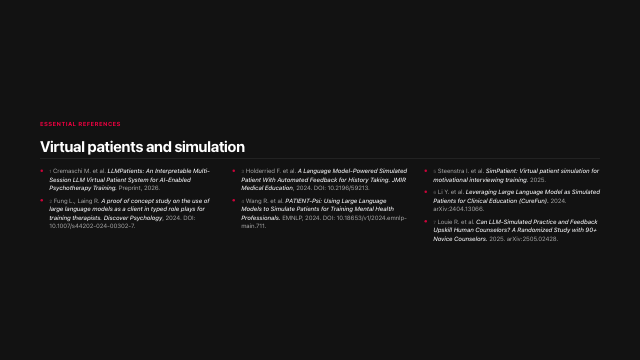
\includegraphics[width=30.4mm]{slides/31.png}}\end{minipage}\hspace{0.5em}
\begin{minipage}[t]{\dimexpr\linewidth-31mm-1.6em\relax}\vspace{0pt}
{\footnotesize\begin{itemize}
\item I will not present this unless someone asks for sources on \textbf{virtual patients} and \textbf{LLM simulation}.
\end{itemize}}
\end{minipage}
\end{minipage}
\vspace{0.45em}\hrule\vspace{0.45em}
\noindent\begin{minipage}{\linewidth}
{\normalsize\bfseries\textcolor{Accent}{Slide 32}}\par
\vspace{0.15em}
\begin{minipage}[t]{31mm}\vspace{0pt}\fcolorbox{Rule}{white}{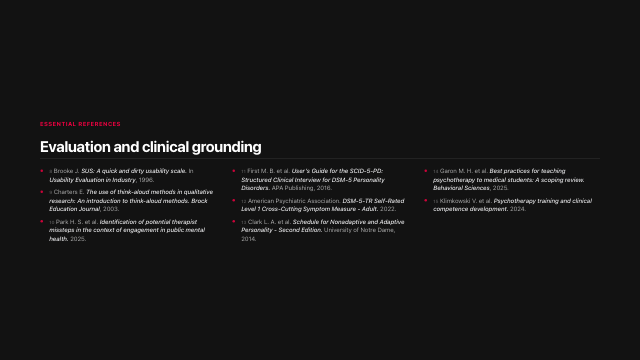
\includegraphics[width=30.4mm]{slides/32.png}}\end{minipage}\hspace{0.5em}
\begin{minipage}[t]{\dimexpr\linewidth-31mm-1.6em\relax}\vspace{0pt}
{\footnotesize\begin{itemize}
\item These are the main references for \textbf{usability}, \textbf{clinical grounding}, \textbf{instruments}, and \textbf{psychotherapy training}.
\end{itemize}}
\end{minipage}
\end{minipage}
\vspace{0.45em}\hrule\vspace{0.45em}
\noindent\begin{minipage}{\linewidth}
{\normalsize\bfseries\textcolor{Accent}{Slide 33}}\par
\vspace{0.15em}
\begin{minipage}[t]{31mm}\vspace{0pt}\fcolorbox{Rule}{white}{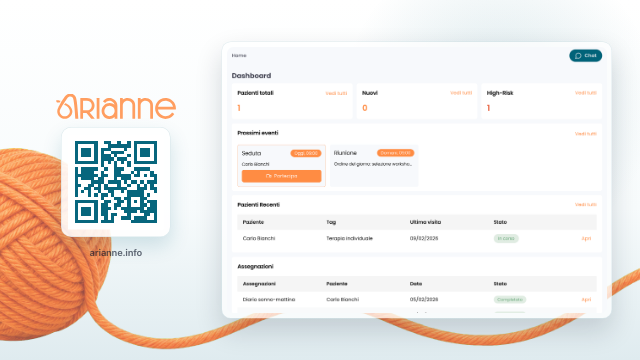
\includegraphics[width=30.4mm]{slides/33.png}}\end{minipage}\hspace{0.5em}
\begin{minipage}[t]{\dimexpr\linewidth-31mm-1.6em\relax}\vspace{0pt}
{\footnotesize\begin{itemize}
\item This \textbf{QR code} opens the \textbf{Arianne website}.
\end{itemize}}
\end{minipage}
\end{minipage}
\vspace{0.45em}\hrule\vspace{0.45em}
\end{document}
